% =====================================================================
% Draft 2 SKELETON: "Reading the Other Document"
% A Rationale-Grounded Mismatch Taxonomy for Android Privacy Disclosures.
% Companion paper to draft-01. Shares the DataGuard corpus.
% Target: International Journal of Human-Computer Studies.
% Build: pdflatex -> bibtex -> pdflatex -> pdflatex
% =====================================================================
\documentclass[11pt,a4paper]{article}

\usepackage[utf8]{inputenc}
\usepackage[T1]{fontenc}
\usepackage{lmodern}
\usepackage{microtype}
\usepackage[margin=2.4cm]{geometry}
\usepackage{graphicx}
\usepackage{xcolor}
\usepackage{booktabs}
\usepackage{array}
\usepackage{caption}
\usepackage{enumitem}
\usepackage{tikz}
\usepackage{pgfplots}
\usepackage{amsmath,amssymb}
\usepackage{url}
\usepackage[hidelinks]{hyperref}
\usepackage[round]{natbib}
\bibliographystyle{plainnat}

\pgfplotsset{compat=1.18}
\usetikzlibrary{arrows.meta,positioning,shapes.geometric,fit,calc,
                patterns,backgrounds,shadows}

% --- Shared colour palette
\definecolor{dgBlue}   {RGB}{ 39, 99,178}
\definecolor{dgBlueL}  {RGB}{218,232,248}
\definecolor{dgOrange} {RGB}{226,123, 32}
\definecolor{dgOrangeL}{RGB}{252,229,205}
\definecolor{dgGreen}  {RGB}{ 84,156, 84}
\definecolor{dgGreenL} {RGB}{225,243,217}
\definecolor{dgPurple} {RGB}{132, 76,162}
\definecolor{dgPurpleL}{RGB}{233,221,242}
\definecolor{dgRed}    {RGB}{200, 64, 64}
\definecolor{dgRedL}   {RGB}{248,215,218}
\definecolor{dgTeal}   {RGB}{ 38,140,140}
\definecolor{dgTealL}  {RGB}{211,236,236}
\definecolor{dgGold}   {RGB}{218,165, 32}
\definecolor{dgGoldL}  {RGB}{251,236,196}
\definecolor{dgGrey}   {RGB}{ 90, 90, 90}
\definecolor{dgGreyL}  {RGB}{235,235,235}

\newcommand{\dataguard}{\textsc{DataGuard}}
\newcommand{\code}[1]{\textsf{#1}}

\title{\bfseries Reading the Other Document: \\
A Rationale-Grounded Mismatch Taxonomy \\
for Android Privacy Disclosures}
\author{Anonymous Author(s)\\\small (Skeleton draft for IJHCS submission)}
\date{}

\begin{document}
\maketitle

\begin{abstract}
\noindent
\textbf{Skeleton draft.} An Android app discloses its data practices
through a structured Google Play Data Safety label and through a long
free-text privacy policy. We use the \dataguard{} audit corpus
($1{,}506$ judgments over $1{,}214$ apps with $1{,}441$ free-text
rationales) to induct a $7$-code taxonomy of label--policy mismatch types
through reflexive thematic
analysis~\citep{braun2006using,wilson2016creation}, validate it against
the inter-annotator-agreement signal, and report the prevalence of each
code across $12$ Google Play categories. The taxonomy gives researchers,
regulators and tool builders a shared vocabulary for the kinds of
mismatch that currently get collapsed into a single ``incorrect'' label,
and motivates code-aware ambiguity indicators in future evidence-grounded
privacy UIs.
\end{abstract}

\noindent\textbf{Keywords:}\ privacy labels; Data Safety; mismatch
taxonomy; thematic analysis; Android; usable privacy.

\bigskip\hrule\bigskip

% =====================================================================
\section{Introduction}\label{sec:intro}
% =====================================================================
\paragraph{The other document.}
A Google Play app ships two privacy artefacts: a short structured Data
Safety table~\citep{googledatasafety2022} and a long natural-language
privacy policy~\citep{mcdonald2008cost,fabian2017large}. Recent
measurement studies show that the two often disagree --- both for Apple
labels~\citep{xiao2023lalaine} and for Google Data
Safety~\citep{khandelwal2024unpacking}. But ``disagree'' is itself a
vague label. Some mismatches are clean contradictions; most are
\emph{kinds} of mismatch with characteristic linguistic markers.

\paragraph{Contribution.}
We induct a $7$-code \emph{Mismatch Taxonomy} from $1{,}441$ free-text
rationales produced by trained annotators inside the
\dataguard{} audit interface (see Draft~$1$). For each code we report:
(i)~its prevalence across $12$ Google Play categories, (ii)~its
\emph{ambiguity score} based on inter-annotator agreement when the code
is invoked, and (iii)~the interface requirement it motivates.

% --- Figure: the 7-code taxonomy ring (placeholder shell)
\begin{figure}[t]
\centering
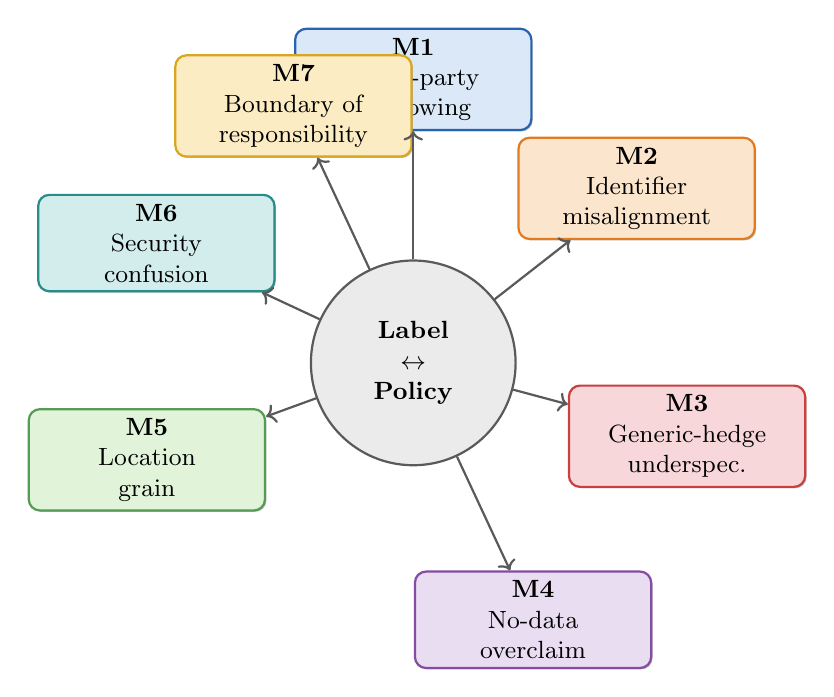
\begin{tikzpicture}[
  every node/.style={font=\small},
  hub/.style={draw=dgGrey,fill=dgGreyL,thick,circle,
              minimum size=2.6cm,align=center},
  code/.style={draw,thick,rounded corners=4pt,
               minimum width=3.0cm,minimum height=1.0cm,align=center,
               drop shadow={shadow xshift=0.5pt,shadow yshift=-0.5pt}}
]
\node[hub] (H) at (0,0) {\textbf{Label}\\$\leftrightarrow$\\\textbf{Policy}};
\node[code,draw=dgBlue,  fill=dgBlueL]   (M1) at ( 90:3.6) {\textbf{M1}\\Third-party\\shadowing};
\node[code,draw=dgOrange,fill=dgOrangeL] (M2) at ( 38:3.6) {\textbf{M2}\\Identifier\\misalignment};
\node[code,draw=dgRed,   fill=dgRedL]    (M3) at (-15:3.6) {\textbf{M3}\\Generic-hedge\\underspec.};
\node[code,draw=dgPurple,fill=dgPurpleL] (M4) at (-65:3.6) {\textbf{M4}\\No-data\\overclaim};
\node[code,draw=dgGreen, fill=dgGreenL]  (M5) at (200:3.6) {\textbf{M5}\\Location\\grain};
\node[code,draw=dgTeal,  fill=dgTealL]   (M6) at (155:3.6) {\textbf{M6}\\Security\\confusion};
\node[code,draw=dgGold,  fill=dgGoldL]   (M7) at (115:3.6) {\textbf{M7}\\Boundary of\\responsibility};
\foreach \i in {M1,M2,M3,M4,M5,M6,M7}
  \draw[->,thick,dgGrey] (H) -- (\i);
\end{tikzpicture}
\caption{Skeleton view of the $7$-code Mismatch Taxonomy.}
\label{fig:taxonomy}
\end{figure}

% =====================================================================
\section{Related work}\label{sec:rw}
% =====================================================================
\paragraph{Automated label--policy mismatch.}
PolicyLint detects within-policy
contradictions~\citep{andow2019policylint};
PoliCheck adds entity-sensitive flow
checks~\citep{andow2020policheck}; MAPS scales the analysis to a million
apps~\citep{zimmeck2019maps,zimmeck2017automated}. Lalaine measured Apple
label compliance at scale~\citep{xiao2023lalaine}; Khandelwal et al.
report on Google Data Safety including a developer
study~\citep{khandelwal2024unpacking}, and an Android/iOS label
comparison~\citep{khandelwal2023comparing}. These works are automated;
ours is human-rationale-grounded.

\paragraph{Vagueness and ambiguity in privacy text.}
\citet{bhatia2016theory} formalise a theory of vagueness in privacy
text; the OPP-115 corpus~\citep{wilson2016creation} shows that
fine-grained policy annotations have moderate agreement;
\citet{rao2016expecting} document mismatched user expectations.
\paragraph{Thematic analysis.}
We use the reflexive thematic-analysis protocol
of~\citet{braun2006using}.

% =====================================================================
\section{Data and method}\label{sec:data}
% =====================================================================
\paragraph{Corpus.} $1{,}506$ judgments, $1{,}441$ rationales,
$1{,}214$ unique apps, seven annotators, $12$ categories. See Draft~$1$
for full provenance.
\paragraph{Sampling.} Stratified random sample of $\sim 200$ rationales
balanced across (judgment-type $\times$ category $\times$ agreement
status $\times$ no-data flag).
\paragraph{Coding protocol.} Two coders independently coded an initial
pilot of $30$ rationales, refined the codebook over two rounds, coded
the remainder, computed Cohen's $\kappa$ on codes, and resolved
disagreements through discussion. We follow the six phases
of~\citet{braun2006using}.

% =====================================================================
\section{The Mismatch Taxonomy}\label{sec:taxonomy}
% =====================================================================
\paragraph{M1 Third-party flow shadowing.} The policy names analytics
SDKs, advertising vendors or named third parties; the label declares no
sharing or omits the relevant categories.
\paragraph{M2 Identifier-category misalignment.} The policy mentions
advertising ID, IP, MAC, SIM or cookies; the label does not include
\emph{Device or other IDs}, or includes it without identifying the
specific identifier.
\paragraph{M3 Generic-hedge underspecification.} The policy uses
``may collect'', ``including but not limited to'', or similar hedges
that leave the actual practice unverifiable.
\paragraph{M4 No-data overclaim.} The label declares no shared and/or
no collected data, yet the policy discusses analytics, ads or service
providers.
\paragraph{M5 Location-grain mismatch.} The policy references coarse,
IP-derived or city-level location; the label does not include a Location
field, or vice versa.
\paragraph{M6 Security-control / data-type confusion.} Security
practices (encryption, deletion) are reported as if they were data-type
disclosures.
\paragraph{M7 Boundary-of-responsibility mismatch.} The policy explicitly
defers responsibility to third-party links, sites or apps; the label
scope becomes ambiguous.

% =====================================================================
\section{Quantitative prevalence}\label{sec:prev}
% =====================================================================
\paragraph{Skeleton.} (i)~Overall prevalence: bar chart of $7$ codes.
(ii)~Per-category $12\times 7$ heat-map. (iii)~Ambiguity-vs-prevalence
scatter where each point is a code; $x$-axis~$=$ fraction of pairs
disagreeing when the code is present.

% =====================================================================
\section{Design implications}\label{sec:design}
% =====================================================================
Code-aware UIs: each code suggests a specific UI affordance --- a third-party
recipient panel for M1, an identifier-mapping helper for M2, a hedging
highlighter for M3, a no-data audit prompt for M4, a location-grain
overlay for M5, a security-vs-data tab for M6, a responsibility-scope
indicator for M7.

% =====================================================================
\section{Discussion and limitations}\label{sec:disc}
% =====================================================================
The skeleton acknowledges that prevalence estimates derive from a
non-representative annotator pool and that the taxonomy is inducted,
not validated against an independent corpus. Future work should
replicate the coding on an iOS Privacy-Label corpus and on a
European/regulator audit panel.

% =====================================================================
\section{Conclusion}\label{sec:concl}
% =====================================================================
We give the field a shared vocabulary for label--policy mismatch and a
prevalence map that turns ``incorrect'' into seven actionable codes.

\bibliography{../draft-01-auditability-gap/references}

\end{document}
